The human brain is anatomically a conglomeration of different brain regions. Functionally, the human brain is a giant network of specialised units connected by dynamically configurable communication pathways. \cite{faes2012methodological}

There are several reasons why scientists would want to measure the way the brain is connected. Understanding brain connectivity aids our knowledge of the working of the brain. It allows us to better understand sensorimotor and cognitive tasks that are performed. This can lead to improved diagnosing of various diseases such as aphasia. \cite{horwitz2003elusive}

A connectivity analysis refers to any analysis where multiple signals are utilised at the same time. The signal can represents several different sources. The signals could be the recordings from different electrodes or, in the case of this thesis, the source-reconstructed EEG data. 

\section{Connectivity Measures}

Different connectivity measures can highlight different aspects about the connectivity. This means that there is not one superior connectivity method. The different connectivity measures are: \cite{friston2011functional, cohen2014analyzing}

\begin{itemize}
\item Phase-Based Connectivity
\item Power-Based Connectivity
\item Cross-Frequency Coupling
\item Graph Theory
\item Granger Causality
\item Information Theory
\end{itemize}

\subsection{Phase-based Connectivity}

Phase-based connectivity analyses utilise the phase differences between different signals. This is a very popular connectivity measure and this is partly because it has a strong neurophysiological interpretation. The timing of neural populations, as measured through phase, become synchronized. This method is computationally fast, does not make many assumptions on the data and is insensitive to time lag. However, it relies on precise temporal relationships.

\subsection{Power-based Connectivity}

Power-Based Connectivity analyses utlise time-frequency power correlations. These correlations are computed accross time or over trials. Power-Based Connectivity analyses are fairly resistant against temporal noise.

\subsection{Cross-Frequency Coupling}

Cross-Frequency Coupling is a statistical relationship between signals in different frequency bands. When utilised on electrodes, it can infer local connectivity when measured at a single electrode. With multiple electrodes, longer-range connectivity can be inferred. One advantage is that findings can be linked across species. Cross-frequency coupling is also very strong at identifying task-related high-frequency power. Computationally speaking, there are some disadvantages to cross-frequency coupling. The search space is huge, which makes it computationally very expensive.

\subsection{Graph Theory}

Graph Theory is a mathematical framework for studying graphs. A graph, containing vertices and edges, can be used to model networks. These networks can be models for brain connectivity. When electrode signals are used, each node can represent an electrode and connectivity is represented by edges. Graph-theoretical analyses are often easy to interpret. Graph theory presents a generic framework to analyse networks, making it easy to apply the same analyses to different kinds of data. The main task becomes the construction of a network. Graph theory is relatively new in the context of computational neuroscience. This makes graph theory an interesting research direction, but this is also a disadvantage. Since graph theory within computational neuroscience isn't as well established, it can be difficult to compare findings to different studies.

\subsection{Granger Causality}

Granger Causality is a statistical method that utilises signal variance. It tests whether variance from one signal can predict variance in another signal at a certain point in time. One big advantage to granger causality is that it can find directional connectivity. It can ignore simultaneous connectivity. This makes it less susceptible to volume conduction. Granger causality is a computationally expensive method to perform. \cite{bressler2011wiener}

\subsection{Information Theory}

Information theory is the main focus of this thesis. It is a simple, yet flexible and robust method for computing connectivity. One useful aspect from information theory is mutual information. Mutual information computes shared information between two variables. This computation is based on the (joint) distributions of values within variables. Information theory has several advantages. It can detect multiple kinds of relationships between different signals. It can detect both linear and non-linear relationships. Information theory also contains many different constructs which are useful for a connectivity analysis. Mutual information is one of them. Another is multivariate generalisations of mutual information, which can work with more than two signals. Channel-coding theory can be used for signal transmission integrity. 

Mutual information is, by far, the most popular method from information theory. One disadvantage is that mutual information does not provide any information on what kind of relationship there is between variables. Information theory is generally defined for discrete distributions, with different techniques to discretize continuous data. However, the method and the chosen parameters for discretizing continuous data have a big effect on the computed results. Information theory is generally also a computationally expensive operation to perform. Finally, there are no clear neurophysiological interpretations for information theoretical constructions. Information theory is discussed much more in-depth in the following chapter, chapter~\ref{information-theory}.

\section{Connectivity Interpretation}

There are several key aspects to keep in mind when interpreting results from a connectivity analysis. Different connectivity measures may or may not take these aspects into consideration. In order to provide a proper connectivity analysis, these key aspects and the properties of the connectivity measures need to be known.

Typically, two different signal are not fully in sync. When an analysis is performed on the signal from multiple electrodes, there may be a phase lag between these electrodes. Most connectivity measures do not take this phase lag into consideration. This does not mean that that these connectivity measures cannot be used, as long as the phase lag is consistent. \cite{horwitz2003elusive}

Figure~\ref{timelag} shows a second key aspect. In this example, region C is connected with A and B. Because C$\rightarrow$A is faster than C$\rightarrow$B, it may appear that there is a phase lag, even though there is no causal or direct relation between A and B.

\begin{figure}[!htb]
\caption{Time Lag \cite{cohen2014analyzing}.}
\label{timelag}
    \centering
    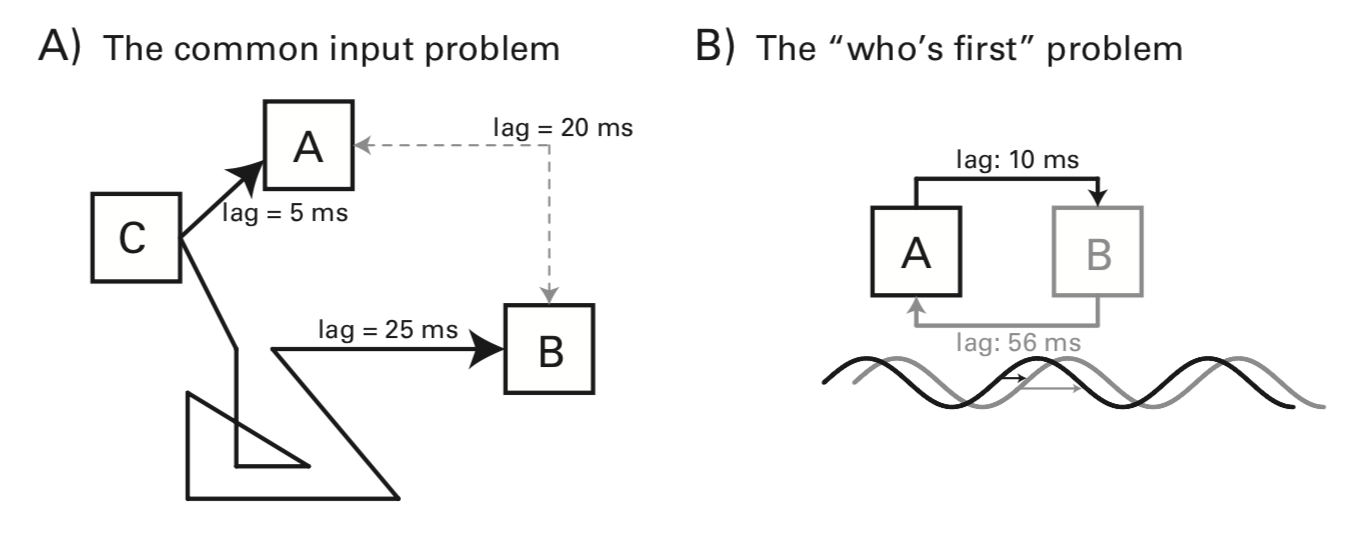
\includegraphics[width=\textwidth]{fig/timelag}
\end{figure}

\section{Volume Conduction}

The head volume conductor model, discussed in chapter~\ref{source-reconstruction}, is quite interesting. The brain conducts electrical activity, this is how the electrical activity can be measured on the scalp. Volume conduction refers to this process of conducting electrical activity through a medium. \cite{brunner2016volume}

Figure~\ref{conduction} shows several problems that the reverse problem has to deal with. In situation A, there would be no problem. In this situation, every EEG electrode measures one and only one electrical source within the brain. However, this is not what happens in reality. 

\begin{figure}[!htb]
\caption{Volume Conduction \cite{cohen2014analyzing}.}
\label{conduction}
    \centering
    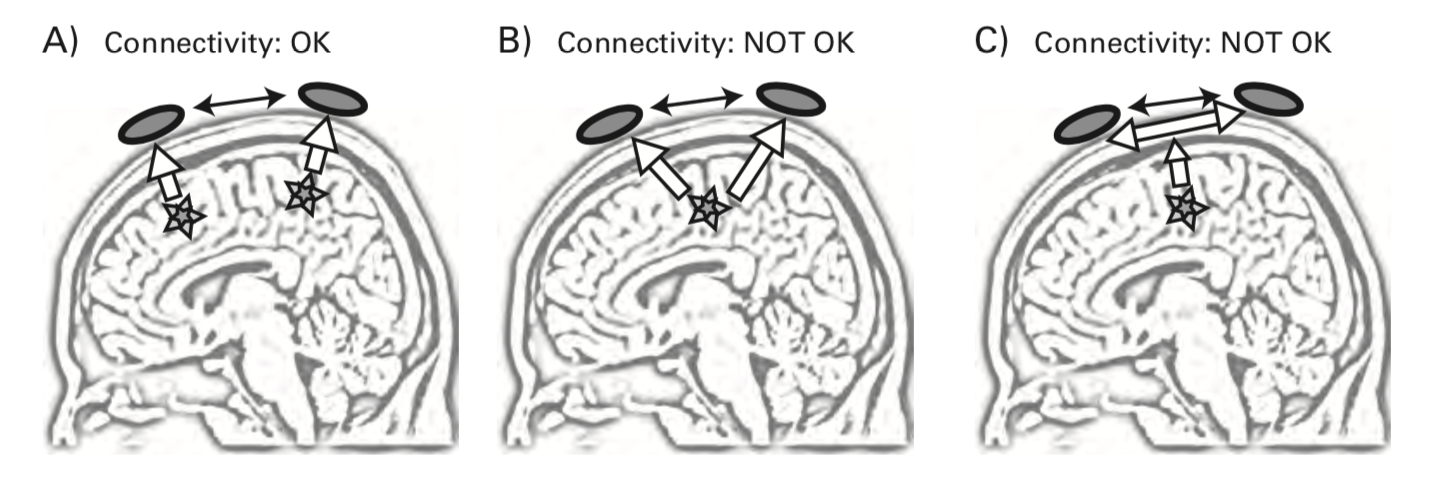
\includegraphics[width=\textwidth]{fig/conduction}
\end{figure}

Reality is a combination of situations B and C \cite{brunner2016volume}. Situation B shows that electrical sources in the brain generate large electromagnetic fields which are recorded by more than one EEG electrode. Situation C shows that the scalp also conducts electricity. These two situations have a big effect on connectivity measures. 
